% L15a figure: what Heun's method and the classical fourth-order Runge-Kutta
% method (RK4) do in one step, for one state variable.
%
% Both panels take the step of Fig-Euler-Steps panel (a): the model
% dx/dt = 1 - x, the computed state 0.2 at t_k, and a step of 0.9 time units.
% The blue curve is the exact solution through that state,
% x(t) = 1 - 0.8 exp(-(t - t_k)), with x(t_{k+1}) = 0.6747.
%   (a) Heun: k1 = 0.8. The Euler trial state is 0.2 + 0.9(0.8) = 0.92 at
%       t_{k+1}, where k2 = 0.08. The average slope is 0.44, and the step ends
%       at 0.2 + 0.9(0.44) = 0.596.
%   (b) RK4: k1 = 0.8; the first midpoint trial state is 0.2 + 0.45(0.8) = 0.56,
%       where k2 = 0.44; the second is 0.2 + 0.45(0.44) = 0.398, where
%       k3 = 0.602; the end trial state is 0.2 + 0.9(0.602) = 0.7418, where
%       k4 = 0.2582. The weighted slope is (k1 + 2 k2 + 2 k3 + k4)/6 = 0.5237,
%       and the step ends at 0.2 + 0.9(0.5237) = 0.6713.
% Each red stage bar is centered on the state where its slope is evaluated and
% spans 0.14 time units.
%
% Layout: both panels use the axis box, the scale, and the title baseline of
% Fig-Euler-Steps panel (a), so the three single steps can be compared.
%
% Drawn on November 27, 2026 with the palette and build of Fig-Euler-Steps.
% The notebook SVG carries a dark palette added by theme_svg.py; keep new colors
% in that script's mapping when changing the palette here.
\documentclass[tikz,border=4pt]{standalone}
\usepackage{amsmath}
\usepackage[no-math]{fontspec}
\IfFontExistsTF{Arial}{\setsansfont{Arial}}{\setsansfont{TeX Gyre Heros}}
\renewcommand{\familydefault}{\sfdefault}
\usetikzlibrary{arrows.meta}

% Blue draws the exact solution, red draws the stage slopes and the step that
% the method takes, and gray draws the trial lines and the guides.
\definecolor{vnink}{HTML}{202124}
\definecolor{gdblue}{HTML}{0091FF}
\definecolor{evred}{HTML}{D93025}
\definecolor{gdgray}{HTML}{6D7278}

\newcommand{\hx}{\hat{\mathbf{x}}}
\newcommand{\kk}[1]{\mathbf{k}_{#1}}

\tikzset{
  axis/.style={draw=vnink, line width=0.6pt, -{Stealth[length=2mm, width=1.6mm]}},
  tick/.style={draw=vnink, line width=0.6pt},
  ticklab/.style={text=vnink, font=\small, anchor=north},
  axlab/.style={text=vnink, font=\sffamily\small},
  exact/.style={draw=gdblue, line width=1.3pt},
  trial/.style={draw=gdgray, line width=0.9pt, dash pattern=on 3pt off 2pt},
  stage/.style={draw=evred, line width=2.4pt, line cap=round},
  rkstep/.style={draw=evred, line width=1.3pt, -{Stealth[length=2.6mm, width=2mm]}, shorten >=3.4pt},
  guide/.style={draw=gdgray, line width=0.5pt, dash pattern=on 1pt off 2pt},
  lab/.style={text=vnink, font=\small, inner sep=1.5pt},
  bluelab/.style={text=gdblue, font=\small, inner sep=1.5pt},
  redlab/.style={text=evred, font=\small, inner sep=1.5pt},
  graylab/.style={text=gdgray, font=\small, inner sep=1.5pt},
  title/.style={text=vnink, font=\sffamily\bfseries, anchor=base},
  startdot/.style={fill=vnink, draw=none},
  reddot/.style={fill=evred, draw=none},
  trialdot/.style={fill=white, draw=gdgray, line width=0.9pt},
}

% \stagebar{t}{x}{slope}: a short red bar with the given slope, centered at (t, x)
\newcommand{\stagebar}[3]{%
  \draw[stage] ({#1 - 0.07}, {#2 - 0.07*#3}) -- ({#1 + 0.07}, {#2 + 0.07*#3});}

% The axes, the time ticks, the exact solution, and its label, shared by both
% panels. Each scope's shift puts the axis corner (-0.15, 0.1) on the baseline.
\newcommand{\panelframe}[1]{%
  \draw[axis] (-0.15, 0.1) -- (1.32, 0.1) node[axlab, anchor=north east, yshift=-2pt] {Time};
  \draw[axis] (-0.15, 0.1) -- (-0.15, 1.06) node[axlab, anchor=south] {State};
  \foreach \t/\name in {#1} {
    \draw[tick] (\t, 0.1) -- (\t, 0.088);
    \node[ticklab] at (\t, 0.083) {$\name$};
  }
  \draw[guide] (0, 0.1) -- (0, 0.2);
  \draw[exact] plot[domain=-0.1:1.2, samples=80, variable=\t] ({\t}, {1 - 0.8*exp(-\t)});
  \node[bluelab, anchor=south east] at (1.32, 0.795) {exact solution};
}

\begin{document}
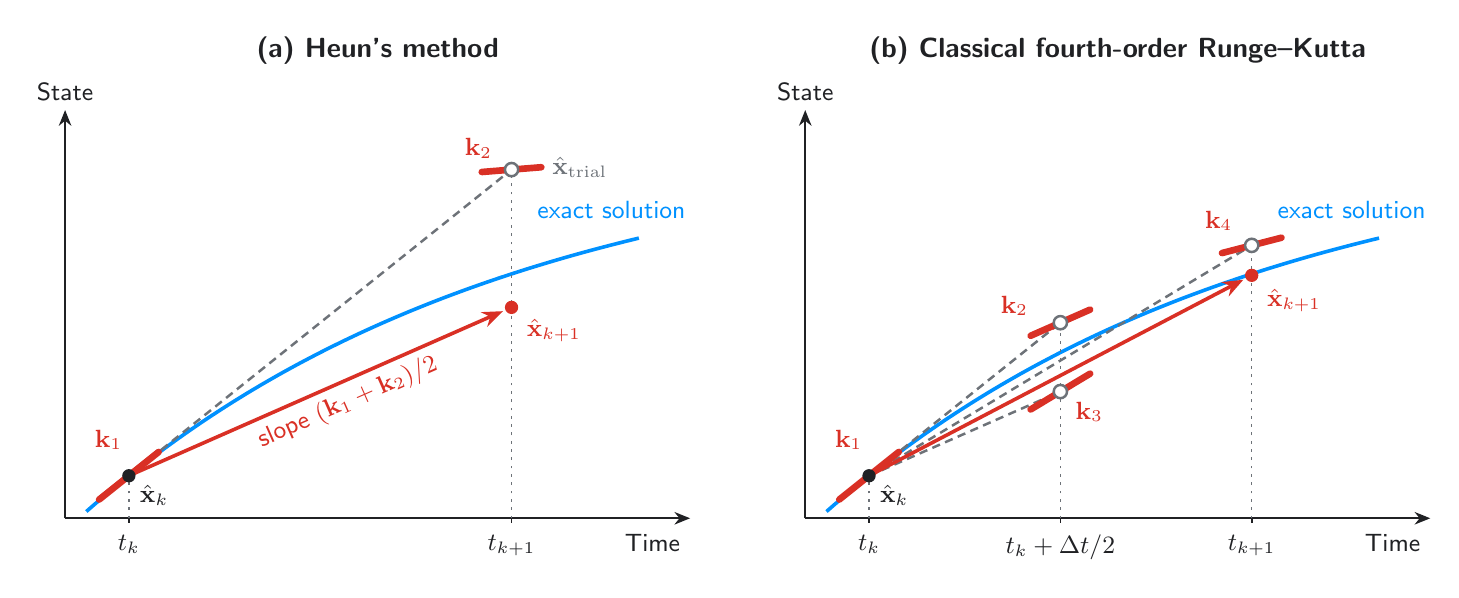
\begin{tikzpicture}

% The two titles share one baseline above the axis boxes.
\node[title] at (3.97, 5.85) {(a) Heun's method};
\node[title] at (13.37, 5.85) {(b) Classical fourth-order Runge–Kutta};

% ------------------------------------------------------------ (a) Heun
\begin{scope}[shift={(0.81cm, -0.54cm)}, x=5.4cm, y=5.4cm]
  \panelframe{0/{t_k}, 0.9/{t_{k+1}}}
  \draw[guide] (0.9, 0.1) -- (0.9, 0.92);
  % the Euler trial step to the end of the step
  \draw[trial] (0, 0.2) -- (0.9, 0.92);
  % the step with the average slope
  \draw[rkstep] (0, 0.2) -- node[redlab, sloped, below, pos=0.55, yshift=-1pt] {slope $(\kk{1}+\kk{2})/2$} (0.9, 0.596);
  % the two stage slopes
  \stagebar{0}{0.2}{0.8}
  \stagebar{0.9}{0.92}{0.08}
  \node[redlab, anchor=south east] at (-0.005, 0.25) {$\kk{1}$};
  \node[redlab, anchor=south east] at (0.865, 0.935) {$\kk{2}$};
  % the points
  \fill[startdot] (0, 0.2) circle (2.4pt);
  \draw[trialdot] (0.9, 0.92) circle (2.4pt);
  \fill[reddot] (0.9, 0.596) circle (2.4pt);
  \node[lab, anchor=north west] at (0.015, 0.19) {$\hx_k$};
  \node[graylab, anchor=west] at (0.985, 0.926) {$\hx_{\mathrm{trial}}$};
  \node[redlab, anchor=north west] at (0.925, 0.58) {$\hx_{k+1}$};
\end{scope}

% ------------------------------------------------------------ (b) RK4
\begin{scope}[shift={(10.21cm, -0.54cm)}, x=5.4cm, y=5.4cm]
  \panelframe{0/{t_k}, 0.45/{t_k+\Delta t/2}, 0.9/{t_{k+1}}}
  \draw[guide] (0.45, 0.1) -- (0.45, 0.56);
  \draw[guide] (0.9, 0.1) -- (0.9, 0.7418);
  % the trial lines from the computed state, one for each of k1, k2, k3
  \draw[trial] (0, 0.2) -- (0.45, 0.56);
  \draw[trial] (0, 0.2) -- (0.45, 0.398);
  \draw[trial] (0, 0.2) -- (0.9, 0.7418);
  % the step with the weighted slope
  \draw[rkstep] (0, 0.2) -- (0.9, 0.67133);
  % the four stage slopes
  \stagebar{0}{0.2}{0.8}
  \stagebar{0.45}{0.56}{0.44}
  \stagebar{0.45}{0.398}{0.602}
  \stagebar{0.9}{0.7418}{0.2582}
  \node[redlab, anchor=south east] at (-0.005, 0.25) {$\kk{1}$};
  \node[redlab, anchor=south east] at (0.385, 0.565) {$\kk{2}$};
  \node[redlab, anchor=north west] at (0.475, 0.385) {$\kk{3}$};
  \node[redlab, anchor=south east] at (0.865, 0.765) {$\kk{4}$};
  % the points
  \fill[startdot] (0, 0.2) circle (2.4pt);
  \draw[trialdot] (0.45, 0.56) circle (2.4pt);
  \draw[trialdot] (0.45, 0.398) circle (2.4pt);
  \draw[trialdot] (0.9, 0.7418) circle (2.4pt);
  \fill[reddot] (0.9, 0.67133) circle (2.4pt);
  \node[lab, anchor=north west] at (0.015, 0.19) {$\hx_k$};
  \node[redlab, anchor=north west] at (0.925, 0.65) {$\hx_{k+1}$};
\end{scope}

\end{tikzpicture}
\end{document}
